% THIS IS SIGPROC-SP.TEX - VERSION 3.1
% WORKS WITH V3.2SP OF ACM_PROC_ARTICLE-SP.CLS
% APRIL 2009
%
% It is an example file showing how to use the 'acm_proc_article-sp.cls' V3.2SP
% LaTeX2e document class file for Conference Proceedings submissions.
% ----------------------------------------------------------------------------------------------------------------
% This .tex file (and associated .cls V3.2SP) *DOES NOT* produce:
%       1) The Permission Statement
%       2) The Conference (location) Info information
%       3) The Copyright Line with ACM data
%       4) Page numbering
% ---------------------------------------------------------------------------------------------------------------
% It is an example which *does* use the .bib file (from which the .bbl file
% is produced).
% REMEMBER HOWEVER: After having produced the .bbl file,
% and prior to final submission,
% you need to 'insert'  your .bbl file into your source .tex file so as to provide
% ONE 'self-contained' source file.
%
% Questions regarding SIGS should be sent to
% Adrienne Griscti ---> griscti@acm.org
%
% Questions/suggestions regarding the guidelines, .tex and .cls files, etc. to
% Gerald Murray ---> murray@hq.acm.org
%
% For tracking purposes - this is V3.1SP - APRIL 2009

% \documentclass{acm_proc_article-sp}
\documentclass[10pt]{IEEEtran}
\usepackage{graphicx}
\usepackage{subfigure}
\usepackage{color}
\usepackage{url}
\usepackage{citesort}
\usepackage{syntax}
\usepackage{wrapfig}
\usepackage{fancyvrb}


\def\todo#1{\textcolor{red}{\textbf{[TODO:~#1]}}\footnote{TODO:~#1}}

\begin{document}


\title{CloudFlow: Cloud-wide policy enforcement using fast VM introspection}


\author{
    \IEEEauthorblockN{Mirza Basim Baig, Connor Fitzsimons, Suryanarayanan Balasubramanian,\\ Radu Sion and Donald Porter\\ }
    \IEEEauthorblockA{Computer Science, Stony Brook University \\
    \{mbaig,crfitzsimons,sbalasubrama,sion,porter\}@cs.stonybrook.edu}
}


% \author{
% \alignauthor
%   Mirza Basim Baig, Connor Fitzsimons, Suryanarayanan Balasubramanian,\\ Radu Sion and Don Porter\\
%       \affaddr{Computer Science, Stony Brook University}\\
%       \email{\{mbaig,crfitzsimons,sbalasubrama,sion,porter\}@cs.stonybrook.edu}  
% }

\maketitle

\begin{abstract}

Increasingly government and commercial enterprises are considering cloud adoption. 
%
Clouds share hardware resources across a number of software virtual
machines.  While this carries the promise of increasingly efficient hardware 
utilization, it also comes with inherent side-channel vulnerabilities which
can be used to mount attacks that cause undesired information leakage.

This is especially important in infrastructures shared by multiple
regulatory constrained, security-disjoint principals. A classic example is a
financial company with multiple departments under the incidence of Chinese Wall 
style regulatory policies designed to curtail illicit gains and conflicts.

And, while at the individual node level, the prevention of side channels is
hard without sacrificing efficiency, a unique mitigation opportunity exists
cloud-wide.  By reactively enforcing information flow invariants through
run-time introspection and on-demand virtual machine migration we can prevent undesired
node-level side-channels with minimal performance overhead.

In this paper we introduce CloudFlow -- an information flow control
mechanism for OpenStack that deploys a new, fast virtual machine introspection mechanism
(orders of magnitude faster than previous approaches) to efficiently and
transparently enable policy enforcement cloud-wide.

CloudFlow mitigates undesirable side-channels, provides protection against undesirable
information leaks and forms a powerful tool enabling information flow policy 
enforcement at cloud scope. Additionally, CloudFlow has potential uses for cloud management and resource-efficient virtual machine scheduling.

\end{abstract}
%\vspace{-5pt}
% A category with the (minimum) three required fields
%\category{D.4.6}{Operating System}{Security and Protection}
%\vspace{-5pt}
%\terms{Security}
%\vspace{-5pt}
%\keywords{Cloud computing, Policy enforcement, VM Introspection, Information flow control} % NOT required for Proceedings

%introduction
\section{Introduction}
\label{sec:introduction}

%\begin{enumerate}
%\item The flexibility and efficiency of the cloud model has prompted increasing number of users to adopt it for their storage and computation needs.
%\item Clients have different needs and usually large companies have many different departments that need segregation of data and computation. This is usually achieved via Bell-Lapdula and Chinese wall policies.
%\item However in a cloud scenario, co-resident VMs give rise to the problem of involuntary side channels.
%\item We need to provide a mechanism that enables MLS segregation for the cloud. We will implement a cloud-wide invariant that states that no side channels-exist between VMs at different MLS levels.
%\item We present MLS-Cloud, a cloud level MLS mechanism that uses fast virtual machine introspection to efficiently and transparently enable MLS policies across the cloud.
%\item MLS-Cloud mitigates involuntary side-channels and enables enforcement of MLS policies for companies running an in-house cloud.
%
%\end{enumerate}

The flexibility and efficiency of the virtualization based cloud computing
makes it extremely attractive for in-house deployments where companies
set up cloud based data centers and share hardware resources across all
their users. 

Nevertheless, clouds come with a number of new security issues, a primary
one amongst them being the inherent existence of side-channels due to resource-sharing. 

Virtual machines (VMs) sharing the same hardware are
vulnerable to malicious side-channel attacks
\cite{SideCrypto,SideCloud,LastSummer,ScriptlessAttacks,PrimeProbe12} making 
the enforcement of proper cloud-wide information flow control difficult.
Yet, this is a major requirement for (in-house) clouds that may be hosting
workload from different units which should be mutually isolated for
regulatory and security reasons. 

For example, information flow control is an essential part of enforcing
regulatory compliance required in e.g., heavily regulated financial companies
which need to enforce Chinese wall policies to segregate resources used by
different internal departments and provide proof that no conflicts of
interest exist as a result of unwanted information leaks. 

History has shown that self-regulation does not always work \cite{Enron} and as a
result laws have been promulgated \cite{Sox} requiring e.g., the
brokerage and investment arms of the same financial organization to be
separated via a Chinese Wall. Similar regulation governs interactions in
healthcare enterprises, financial ratings companies etc. 

Intra-node and limited inter-node information flow control mechanisms have
been researched for decades and have resulted in several practical systems
such as Histar \cite{HiStar} and SELinux \cite{SeStat} which aim to provide
general MLS and information flow control mechanisms at OS level.

However, since node-level side-channels cannot be eliminated efficiently when
resources are shared across multiple co-resident VMs, it is important to
explore whether and how cloud-wide information flow invariants can be
enforced.

Unfortunately, the explosive emergence of clouds has left its adopters
without access to information flow control tools that work at cloud scope,
and businesses are forced to deploy inefficient, ad-hoc solutions such as
manual segregation of internal networks and hosts to solve their regulatory
compliance information flow control requirements.  Overall, private cloud
technology is missing a security platform that can translate high level
information flow control policies, such as role based user and workflow isolation, 
into micro security decisions that are enforced infrastructure-wide at runtime.

Initial work (Home Alone \cite{HomeAlone}) has tackled certain issues of
side-channel prevention in public clouds by allowing a tenant to verify its
VMs' exclusive use of a physical machine.  

In this paper we go one step further and design a cloud-wide, automatic
information flow control mechanism. CloudFlow is a suite of lightweight
modules designed for OpenStack \cite{OpenStack} that deploy fast
hypervisor-level VM introspection, management and migration
to efficiently and transparently enforce cloud-wide information flow control
invariants. The main philosophy behind CloudFlow is to not require any
changes to the hosted guest VMs or applications.

The main contributions of this work are as follows. Firstly, we provide a
new introspection mechanism for KVM-QEMU \cite{QEMU} that
allows for fast asynchronous VM introspection at the hypervisor
level. Our technique is several orders of magnitude faster than previous 
libraries such as libvirt \cite{libvirt} and libVMI
\cite{libvmi}.  Secondly we design a cloud-wide information flow control
layer for OpenStack \cite{OpenStack} that leverages the introspection
mechanisms to enforce best-effort real-time information flow control.



%Background and threat model
\section{Background and Model}
\label{sec:model}

\begin{figure*}[t]
\begin{center}
\includegraphics[scale=0.5]{figures/cloudflow2.eps}
%\vspace{30pt}
\caption{\small 
% 
Administrators from different departments provide CloudFlow with VM images
and desired security policies.  CloudFlow (CF) deploys the images to the
cloud and propagates CF policies automatically to relevant nodes.  The
policies are then used to dynamically deduce CF labels for VMs.  Policies
are enforced in real-time using VM introspection and call-backs to the management module(e.g. 
migration requests).  The figure shows a migration in progress.
%
\label{cloudflow:figure:highlevelarch}}
\end{center}
\end{figure*}


\paragraph{\bf Regulatory compliance \& Information flow control}
%What are they
%Regulatory compliance and information flow control
%make 1 paragraph out of both of the two belows - > all these things require information flow control

%People do not trust institutions when they believe that the appropriate policies to deter abuse are lacking or not being enforced. When the public trust is threatened, often new regulations and policies are put into place to restore trust. For example, Enron was a leading energy company in the 1990s that went bankrupt in 2001 \cite{Enron}. Enron's pensioners, employees, and ordinary shareholders suffered huge financial losses while Enron's top management made hundreds of millions of dollars from selling stock at prices inflated by fraudulent financial reporting. Instead of stopping the fraud, Enron's accounting auditor, Arthur Andersen, helped carry it out, then tried to destroy the evidence \cite{AP02}. To restore public trust in the financial accountability of publicly-traded corporations, Congress passed the Sarbanes-Oxley Act \cite{Sox} in 2002. To comply with SOX, companies have had to make fairly expensive changes to their IT processes; Congress's intent is that the cost of these changes is much less than the cost to society of not being able to trust corporate financial reports. Similarly, compliance with the Health Insurance Portability and Accountability Act \cite{HIPAA} has been quite expensive, but presumably much less than the societal cost of errors, omissions, and inappropriate disclosure of medical records.

%HIPAA and SOX created markets for new IT products that could increase assurances at reasonable cost. As society increases its reliance on electronic delivery of services from government, business, and educational institutions, new trust issues will continue to arise, and trust-related legislation and opportunities for new technology that increases trust will continue to grow. Already there are many major regulations that address IT trust issues, including the Gramm-Leach-Bliley Act \cite{GLB}, Federal Information Security Management Act \cite{FISMA}, Securities and Exchange Commission (SEC) rule 17a-4 \cite{SEC17cfr241}, Food and Drug Administration 21 CFR Part 11 \cite{FDA21cfr11}, the Family Educational Rights and Privacy Act \cite{FERPA}, the e-Government Act \cite{EGA}, and the Patriot Act \cite{Pat01}.

People do not trust institutions when they believe that the appropriate
policies to deter abuse are lacking or not being enforced.  When the public
trust is threatened \cite{Enron}, often new regulations and policies are put
into place to restore trust.  Over 10,000 IT-impacting regulations exist in
the US alone, including Sarbanes-Oxley Act \cite{Sox}, Health Insurance
Portability and Accountability Act \cite{HIPAA}, Gramm-Leach-Bliley Act
\cite{GLB}, Federal Information Security Management Act \cite{FISMA},
Securities and Exchange Commission (SEC) rule 17a-4 \cite{SEC17cfr241}, the
e-Government Act \cite{EGA}, and the Patriot Act \cite{Pat01}.

%strongly link all of the above to information flow control

The core issue that many of these laws ultimately address is the need for
fair and transparent control of sensitive information.  Accordingly,
information flow control is an essential necessity within any large
organization.  However, with scale come increasing difficulties in enforcing 
information flow control, and illicit accesses can go unmonitored.

%too  many often
\paragraph{\bf MLS and Chinese Wall policies}
%
Of particular importance in regulatory contexts are Chinese Wall policies
that institutions need to enforce to mitigate existing and potential
conflicts of interest.  A \textit{Chinese Wall} is a barrier placed
across information flow within an organization that aims to segregate
employees who have access to sensitive information from those who may
use this information for personal gain.  Traditionally this is
done by isolating personnel from each other and monitoring information
access and sharing.  As we will see, CloudFlow can naturally enforce Chinese
wall policies by dynamic inter-VM segregation for applications running on
behalf of principals under regulatory constraints.

% MLS systems process information with differing, often incompatible,
% security levels.  They provide access control mechanisms for users at
% different security clearances and needs-to-know, and thus prevent
% illegitimate access to information.

Similarly, in intelligence and defense scenarios, information flow control
is subject to \textit{Multilevel security} (MLS) policies.  MLS systems
process information that exists at differing, often incompatible, security
or \textit{classification levels} and provide access control mechanisms for
users at different security clearances and needs-to-know, preventing
illegitimate access to classified information.  One popular example 
is the well known Bell-Lapadula confidentiality policy model
\cite{BellLapadula}.  Traditionally, Bell-Lapadula uses four different
classification levels, from Top Secret down to Unclassified. Information
flow is controlled according to ``no reads up, no writes down'' rules. 
% incorrect:
% Other MLS models, such as the Biba model \cite{Biba}, exist
% for enforcing data integrity instead of confidentiality.  
CloudFlow can also naturally enforce MLS policies as will be shown later.

There has been previous work on network-centric cloud-wide policy
enforcement \cite{CloudEncPolicy10,NetODESSA,CloudProfit12,CloudPower12,AllocationPolicy10}. Policies are usually defined in order to attain better
segregation amongst nodes of different computational and storage needs and
provide better load balancing or scheduling algorithms.  Work that most
closely resembles CloudFlow includes a result that proposes stronger VM isolation
mechanisms \cite{Mushi}.  Such mechanisms rely mainly on providing
rudimentary MLS via hardwired network isolation.


\paragraph{\bf Side Channels}
%Side channels exist wherever you have information leakage

\begin{wrapfigure}{L}{0.16\textwidth}
\vspace{-10pt}
\includegraphics[width=0.20\textwidth]{figures/memh2.eps}
\vspace{-25pt}
\label{cloudflow:figure:memh}
\end{wrapfigure}

% An organization that has information flow control procedures in place may
% still be susceptible to information leakage via \textit{side channel
% attacks}.  
In a {\em side channel attack} information is gained
from a system using a resource that is shared between an unsuspecting victim and a perpetrator.  Examples of such shared resources include power conduits, discs, shared memory hierarchies etc. all of which can be used to infer potentially sensitive information illegitimately.

An especially important and interesting class of side channels arises due to
improper VM isolation.  This derives from the inherent resource sharing
design that comes with efficient infrastructures.  For example, clouds
usually multiplex multiple VMs on the same underlying hardware by assigning
a virtual CPU (VCPU) to each VM.  The number of VCPUs can be greater than
the physical CPUs and hence, in the case of load balancing a large number of
VMs, different VCPUs end up getting mapped to the same physical CPU.  Two
VMs on the same physical CPU end up sharing all levels of the memory
hierarchy.  This can lead to information leakage e.g.,  via shared caches
\cite{SideCloud,SideCrypto}.  Even though the two VMs share no explicit
state, the CPU cache is a shared resource impacted by the internal state of
both VMs (see Figure).  This
introduces a side channel that potentially breaks desired information flow
control invariants.  Numerous other side channels have been discovered in a
variety of settings and have been studied extensively
\cite{SideCloud,SideCrypto,LastSummer,ScriptlessAttacks}.  Associated
exploits have been designed and implemented to extract private information
such as RSA and AES keys \cite{SideCloud,SideCrypto,PrimeProbe12} via side channels from
unsuspecting victims.

While preventing individual side channels at OS and hypervisor level is
difficult and arguably impossible to achieve in efficient resource sharing
systems, we believe a unique mitigation opportunity exists at cloud level. 
By reactively enforcing information flow control invariants through runtime
introspection and on-demand VM migration the effects of existing side channels can be mitigated.
However we acknowledge the fact that any system that is reactive in nature can be subject to 
{\em residual side channels} i.e. whenever a policy is enforced at runtime the attacker has the opportunity 
to learn information about the policy being enforced. This is not an issue in the regulatory compliance scenario 
under focus in this paper as policies themselves are not classified information and do not need to be protected from side channel attacks.
% Thus our technique is preventive in nature.

\paragraph{\bf VM Introspection}

Introspection was
first suggested in the seminal work of Garfield and Rosenblum \cite{Terra}. 
Two types of introspection mechanisms exist: those requiring changes to the
guest VM or target applications, and those that work externally at the hypervisor level.  CloudFlow aims for maximum
transparency and minimizing the impact on guest OSes and applications and
thus uses external introspection.

Introspection has been extremely popular in the recent past
\cite{RemoteAttestation,OutOfBox,OutOfBoxMalware,AntFarm,VMIObserve,TamperResist,libvmi}. 
Previous introspection mechanisms have been aimed towards solving problems such as intrusion detection \cite{CoPilot}, malware analysis
\cite{Ether} and forensics.  

External introspection approaches however are inherently at a disadvantage
due to having an outsider view and remain prone to the {\em semantic gap}
problem \cite{chen01virtual,SemanticGap}, the difficulty of mapping between
low-level hardware events and higher-level system abstractions.  Further, in
practice, interpreting the memory of a running guest OS can be error prone,
and subject to attacks \cite{DKSM}.

In recent years there has been much effort to reduce this gap and gain
meaningful, detailed information even in the case of non-cooperating,
adversarial guest VMs \cite{Virtuoso,ProcessImplanting}.  This has led to
the construction of hybrid approaches that install an agent inside the monitored
guest as well, to provide a view that is richer in semantics.

%Why are they used
\paragraph{\bf Clouds}
% 
Cloud computing enables the outsourcing of computation and storage needs to
an infrastructure managed by a third party (public cloud provider, or
in-house company-wide cloud/IT department).  Clouds today are mostly
virtualization based i.e.  they use VMs as the basic unit for leasing out
computation.  They usually provide a management front-end which can be used
as an input point to deploy and manage workload-personalized VMs which are
run in a data center composed of physical nodes that provide
computation and storage, and can host multiple VMs simultaneously.  

CloudFlow is based on the OpenStack \cite{OpenStack} framework. OpenStack
offers a variety of services including computing and storage nodes, and
works with a wide range of hypervisors.  OpenStack is research friendly and
provides open source code which facilitated our design.  In addition, we
have picked the popular KVM-QEMU as our hypervisor of choice. Nevertheless we note that CloudFlow is hypervisor agnostic and it can be easily ported to other cloud platforms.

%Insert deployment model here
%who are users. how are labels acquired. what is deployed. what are labels. ideally we want to be able to write policy based on any guest state. however cloudflow currently only looks at labels. why?

\paragraph{\bf Deployment Model}
% 
The key idea behind CloudFlow is to enable hypervisors and the cloud
management layers to dynamically enforce cloud-wide information flow
policies that are based on guest VM state introspected at runtime.  For
example, in the case of Bell-Lapadula/MLS enforcement, a policy may specify
that no VM running applications classified/labeled as "confidential" can be hosted
on the same physical node as a VM running an application handling "top
secret" labeled data. No application and guest OS changes should be required. 

Naturally, the granularity at which guest state can be monitored via
introspection can vary vastly depending on the depth of data extracted from
the monitored kernel.  For illustration purposes, the current version of
CloudFlow allows policies containing references to SELinux labels of
guest-hosted processes.  The set of labels is currently derived from the
typing system put in place by SELinux inside each guest.

\paragraph{\bf Threat Model \& Assumptions}
% 
Of major concern are insiders who will benefit from cross-VM side channels.
Our main insight is that while at individual node level, the prevention
of side channels is tantamount to sacrificing efficiency, at cloud level we
can reactively prevent undesired side channels by intelligent on-demand
policy-enforcing VM placement, without a significant performance hit.

We trust the hypervisor, cloud administrators and policy designers. All
other users are untrustworthy.

Typically attackers will deploy a a malicious VM through which they will
attempt to exploit a known hardware side channel and extract sensitive
information from a unsuspecting target VM.  We assume that the adversary is
not in control of the entire underlying hardware and is unable to
bypass the hypervisor isolation.

Further, while we do not fully trust the guest OS and its applications, we
assume that guest kernels do not aim to subvert the introspection mechanism. 

Nevertheless, we note that recent work \cite{DKSM} has shown it is possible to deceive hypervisor
based introspection mechanisms via an attack on the guest kernel. This is
why ideally the guest OS should be entirely untrusted.

For this reason we designed a framework that can be ultimately independent
of guest support.  Additionally, we note that because CloudFlow does not modify the guest OS it does not need constant maintenance upon every kernel version update. CloudFlow can run on multiple kernel versions and different operating systems by simply changing how the introspection is performed externally. Finally, CloudFlow allows us to set a base for the policy
management and information flow control that remains agnostic of how the
guest state is actually acquired.

In ongoing work we are developing deception-robust introspection mechanisms that can
handle fully malicious guest kernels.

\begin{figure}[t]
\begin{center}
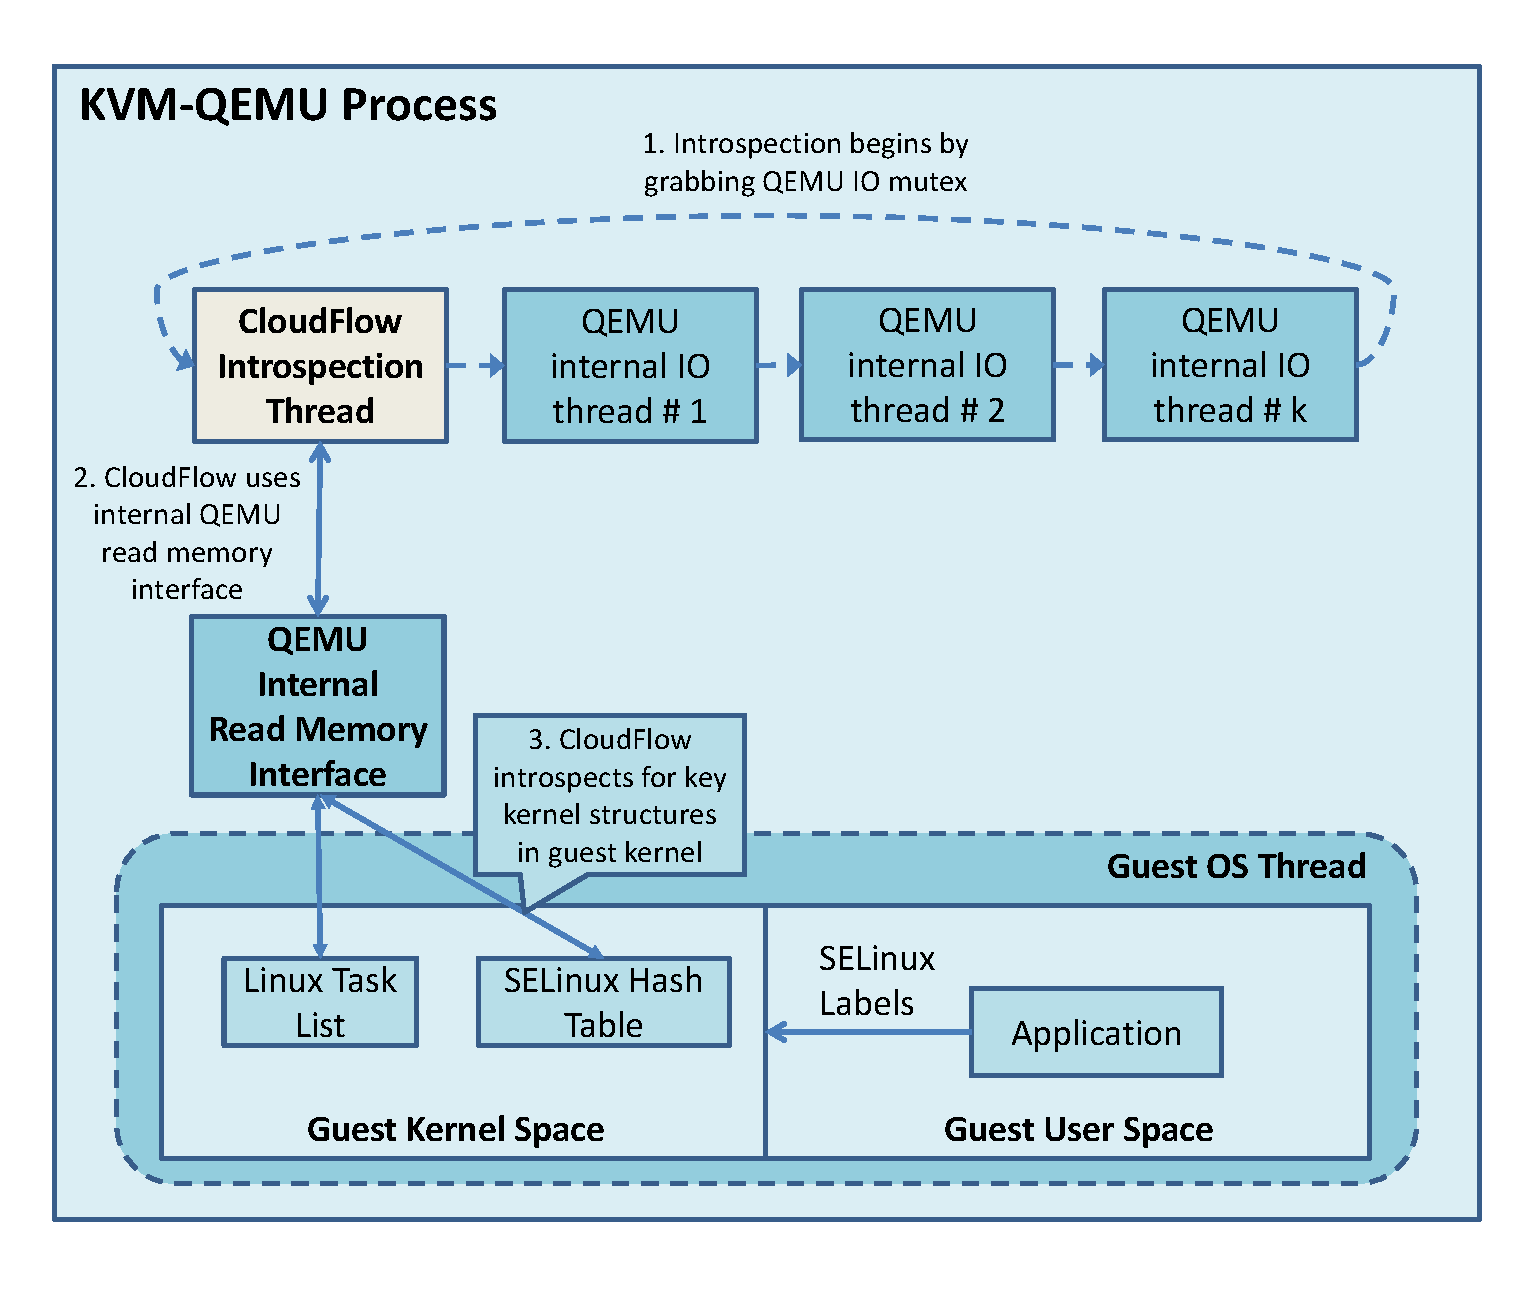
\includegraphics[scale=0.3]{figures/introspectionmodule2.eps}
%\vspace{30pt}
\caption{\small 
%
CloudFlow deploys a fast introspection thread that uses KVM-QEMU internals
directly to extract key kernel structures and infer information about tasks
running inside the guest OS.
%
\label{clowdflow:figure:introspectionmodule}}
\end{center}
\end{figure}



%Architecture/Implementation
\section{Architecture \& Implementation}
\label{sec:architecture}

CloudFlow is a modular system composed of several asynchronously connected
components.  It provides a cloud-wide enforcement mechanism, assisting in
information flow control via active policy deployment and on demand VM
relocation.  CloudFlow only requires VM images and policies as input (Figure
\ref{cloudflow:figure:highlevelarch}).  Policies are propagated to nodes
on-demand at runtime. 
 
During execution, each VM has a set of application-specific labels
associated with its running tasks.  The appearance or disappearance of a
guest-hosted application with a given runtime label may trigger a
policy-defined action.  This action may be null or may result in the
relocation or halting of a subset of VMs.  The ultimate purpose is reactive
defense against any potentially unallowed information flows, as defined by the currently deployed policies.  

CloudFlow can naturally enforce different types of information flow policies
including Chinese Wall and Bell-Lapadula MLS models.  For example in the
case MLS policies, the runtime labels can be thought of as MLS
classification labels and CloudFlow as a runtime MLS enforcement mechanism.
\vspace{5pt}
\subsection{Introspection Module}
% 
CloudFlow deploys VM introspection to extract runtime labels
from key guest kernel data structures.  CloudFlow enforces information flow
in real-time which renders existing introspection libraries for KVM-QEMU
unusable due to their relatively high latency and low speeds.  For these reasons,
CloudFlow undertakes VM introspection by hooking into existing KVM-QEMU
internals and significantly reducing overheads due to unnecessary levels of
indirection added by external libraries.

Introspection is performed by a specialized introspection thread, one instance of which is placed near each monitored VM. 
The introspection thread runs as part of the KVM-QEMU hypervisor code base
\cite{QEMU} and exists inside the KVM-QEMU process.  It inserts itself inside the scheduling chain of hardware I/O threads
(within KVM-QEMU) that manage hardware I/O virtualization for the hypervisor
(Figure \ref{clowdflow:figure:introspectionmodule}).  This allows the use of
KVM-QEMU's internal mechanisms for quick access to guest memory. QEMU uses these mechanisms to manage DMA between I/O threads and the guest operating system however we leverage them for quick introspection. The
introspection thread synchronizes with the other threads using existing
locking mechanisms.  Yet since KVM-QEMU follows a hybrid approach that allows
both multi-threading and event based programming, the introspection
thread is also aware of internal scheduling demands of KVM-QEMU and yields
the I/O lock often enough to allow graceful handling of KVM-QEMU events.

With a hook into the KVM-QEMU's internal guest memory reading interface and
a number of synchronization issues resolved, the introspection thread feeds
from two key guest kernel data structures: the task list and the SELinux
hash table containing context information for all running tasks.  The thread
extracts this information periodically, monitoring for changes to the running
task list and associated SELinux context information.  The
thread receives a list of target labels of interest (from the policy
infrastructure) and continuously searches for them inside the target guest. 
Once a related change happens inside the guest kernel, the information is 
propagated from the guest to the policy checking modules within a few
milliseconds\footnote{This is a vast improvement over latency caused
by using existing introspection libraries as we show in Section
\ref{sec:evaluation}.} (which constitutes a vulnerability window discussed
later). 

Also, for extensibility and re-usability, the introspection thread is
segregated into two separate components.  The first component handles the
interfacing with KVM-QEMU internals, while the second component provides
the SELinux-aware data extraction mechanisms.

Since only the second component is entangled with CloudFlow particulars, the
first component in fact constitutes a new fast introspection interface for
KVM-QEMU which will be made public as a QEMU patch.

\subsection{Policy Language Model}

As previously mentioned, CloudFlow follows a policy-centric approach. Its
policy language provides a way to delineate information flow control
decisions in the form of high level policy constructs a subset of which is shown in Figure \ref{figure:policystructure}.

\begin{figure}[t]
\vspace{-5pt}
\begin{Verbatim}[frame=single]
<policy-list> = <policy>
	      | <policy> <policy-list>

<policy> =  <p> if <label> in <locality> 
                then <action> </p>

<label> = {Set of target runtime labels}

<locality> = <co-resident> | <self>

<action> = <migrate> | <halt> | resume
\end{Verbatim}
\vspace{0pt}
\caption{Subset of CloudFlow Policy Language}
\label{figure:policystructure}
\end{figure}
%add a footnote Obviously arbitrary Turing-complete language could be deployed here.
For simplicity and efficiency purposes we have decided to keep the CloudFlow language as simple as possible\footnote{Obviously any arbitrary Turing-complete language could be deployed here} while still serving as a sound illustrative example. Currently the policy language has a simple grammatical model. Each policy list is made up of one or more policies. Each policy expects a label, the
locality of the target virtual machine and an appropriate action to perform
in case of a positive match for the provided label. Presently, the set of labels is limited to
SELinux \cite{SeStat} types. However it must be noted that even though we use SELinux types as labels, our policies are simple in nature and do need expertise to craft as is the case with SELinux policies. We felt there is value in
coupling with guest SELinux ecosystems, to allow for a wide range of complex
policies, yet not require changes to existing guest logic. We note that the set of labels can be changed arbitrarily along with the underlying OS.

All label symbols form terminal symbols in the policy grammar. The set of localities is formed of two terminal symbols {\textless co-resident\textgreater} and {\textless self\textgreater}. As all policies are written from the viewpoint of a particular VM, this part of the policy outlines whether the label should be searched for in the VM itself (self) or in all the VMs co-resident to it (co-resident). Finally the set of actions is formed of three terminal symbols  {\textless migrate\textgreater}, {\textless halt\textgreater} and {\textless resume\textgreater}. These symbols are pretty self-explanatory as they outline the action that needs to be taken on the VM that contained the label specified by the current policy.

Consider for example
the case when VMs for users Alice and Bob need to be kept physically isolated
throughout the cloud infrastructure -- the corresponding policy for Bob is
illustrated in Figure \ref{cloudflow:figure:examplepolicy}. 
In this example, processes run by Alice are
marked as ``Alice'' (as well with a number of other labels, including the process
name) at runtime by the SELinux subsystem on each guest to facilitate in the introspection process.

Further, we have picked XML as the format of choice for the actual
implementation of the policy files.  The policy language itself
is agnostic to the format used in the implementation.  In fact, early versions of CloudFlow were using key-value pairs to implement the policy language.  XML has a flexible structure
that allows quick extensions with minimal effort. As CloudFlow policies
and associated scenarios mature we envision a set of graphical tools to
manipulate these cloud-wide policies. 

\begin{figure}[h]
%\vspace{0pt}
\begin{Verbatim}[frame=single]
<p> if <Alice> in <co-resident>
    then <migrate> </p>
\end{Verbatim}
\vspace{-10pt}
\caption{Example policy
\label{cloudflow:figure:examplepolicy}}
\end{figure}
\vspace{10pt}

\subsection{Management Module}

The CloudFlow management module is the component that provides an entry
point to the cloud administrator.  An administrator can input a VM image
along with a list of security policies written by a policy designer.  In addition to the usual management tasks,
such as deploying and tracking the VMs, the CloudFlow management module does all the
house-keeping such as storing and propagating
policies.  The module is integrated seamlessly in the OpenStack
platform \cite{OpenStack} and features additional code to handle call-backs from the
policy module as well as user interface events.

\subsection{Policy Module (Daemon, Master)}
% 
The CloudFlow management module propagates the provided policies to the
actual policy enforcement infrastructure.  CloudFlow runs a cloud-wide
policy master module (PolicyM) and a per-node instance of the policy daemon
(PolicyD).  PolicyM acts as a master that controls all running instances of
PolicyD and keeps track of conflicts across physical hosts.  Meanwhile,
PolicyD has the job of maintaining policy lists for a given physical node as
well as interfacing with the introspection module for each VM.

\begin{figure}[h]
\begin{center}
\includegraphics[scale=0.3]{figures/moduledesign2.eps}
%\vspace{30pt}
\caption{\small 
%
CloudFlow follows a completely modular design. VM management, policy
enforcement and VM introspection are all performed by dedicated modules.
%
\label{cloudflow:figure:moduledesign}}
\end{center}
\end{figure}

\begin{figure*}[t]
\begin{center}
\includegraphics[scale=0.70]{figures/illustrativepicture.eps}
%\vspace{30pt}
\caption{\small 
%
CloudFlow performs dynamic policy-triggered VM relocation based on input policies. 
An example policy is one that disallows two users (Alice and Bob) from being co-resident 
on the same physical node based on \textit{runtime labels}.
%
\label{cloudflow:figure:illustrativescenario}}
\end{center}
\end{figure*}

Whenever a new policy is passed to PolicyD by the management module at VM
deployment time, it parses target labels in the policy and passes them on to
the appropriate introspection module.  It also notifies PolicyM that a new
VM has become active in the cloud.  Similarly in the case of VM deletion,
PolicyM is informed by PolicyD of the change.  Additionally, whenever a
policy label ``matches'' a runtime label inside a guest VM, PolicyD gets
notified by the corresponding introspection module, in effect ``triggering''
a policy.  PolicyD looks up the required action as specified by this policy.  In case of
a ``halt'' action, PolicyD simply issues a halt call-back to the management
module.  In case of a ``migration'' it issues a request to PolicyM to search for
a potential migration target.

PolicyM maintains high level state for the entire cloud and in case of a
migration request from PolicyD, it scouts for a target node that does not
introduce additional conflicts.  To this end PolicyM executes a
reconnaissance phase to find the potential migration target.  It queries runtime
labels for all deployed VMs from the associated PolicyDs and crosschecks
them with deployed policies.  This allows for the selection of a migration
target that (at least in the immediate future) will not cause further
conflicts.  PolicyM then reports this host back to PolicyD, which issues the
migration request call-back to the management module.  The CloudFlow PolicyD and
PolicyM were written from scratch in Python and Java respectively.



\subsection{Illustrative Scenario}
%make sure illustrative diagram is here
Here we outline an illustrative scenario (Figure \ref{cloudflow:figure:illustrativescenario}). 
Consider a law firm with two clients A and B, handled by employees Alice and
Bob respectively.  State and federal laws prevent Alice and Bob from sharing
any information due to the possibility of a conflict of interest arising. 
In this scenario, CloudFlow prevents an information leakage as follows:




\begin{itemize}

\item A policy is created outlining the fact that workloads run by users
Alice and Bob should not be co-resident.  The simple policy in Figure
\ref{cloudflow:figure:examplepolicy} can be used as an example.  The policy
will be described for Alice and Bob and propagated automatically along with
both their VMs at time of deployment.

\item Sometime in the future Alice is working on client A's data and needs
to run her workload.

\item Bob uses the same cloud as Alice and it just so happens that the cloud
scheduler locates their VMs on the same physical machine {\em before they both
start their respective security-critical workloads}.

\item After some time Alice's VM boots up and launches the desired
Alice-labeled workload. 

\item The introspection thread assigned to Alice's VM will immediately raise a flag
as soon as it notices the Alice label on the applications.  This event is 
sent back to the PolicyD running on the current physical node.  PolicyD
looks at the policies that have been specified for the VM that issued the
call-back.  Although PolicyD finds one policy that specifies Alice, it knows
that currently there are no other VMs on the same machine running workloads
from Bob hence no action is taken.

\item After some more time passes, Bob's VM boots up and launches its
Bob-labeled workload.  At this point the introspection
thread for Bob's VM reports back to PolicyD
having seen the desired runtime label 'Bob'.

\item PolicyD now works out that an administrator has specified a policy
that prohibits the current cloud state (Alice and Bob have co-resident workloads).  Alice's VM is frozen to prevent 
any security breach.

\item The action specified by the policy i.e., migration, is then passed back
to the PolicyM module by PolicyD along with the id for Alice's VM.

\item PolicyM now begins a reconnaissance phase to locate a potential migration target
to relocate Alice's VM.  In this phase PolicyM queries a list of runtime
labels from all potential hosts and as soon as it finds a target host that
will not cause a policy conflict with Alice's VM, it returns the host name
to the PolicyD that issued the migration request.

\item PolicyD, having acquired a conflict-free migration target, issues a
migration request to the management module for relocating Alice's VM..

\item The OpenStack module issues a migrate action, as it normally would for
load balancing, and migrates Alice's VM to the provided migration target,
where the VM resumes.


\end{itemize}



%Discussion
\section{Discussion}

\noindent 
{\bf Information Flow Invariants.~}
We need to caution that any reactive system cannot
be provably secure. 

CloudFlow enacts a best-effort approach that aims to minimize the
vulnerability window during which an attack can be mounted against a target
VM.  In practice however, we observe that the window of vulnerability is so
small (\textless 5ms, Section \ref{sec:evaluation}) that it easily defeats any
existing and foreseeable side-channel attacks which are usually low-bandwidth
and require comparatively ample amount of time to deploy \cite{SideCrypto,SideCloud,PrimeProbe12}
(\textgreater hours).

\noindent
{\bf Users \& Groups.~}
%
CloudFlow allows the straightforward definition and enforcement of user and
group/role-based policies. Roles can be associated with underlying SELinux
labels which can then be used in the policy definitions. 

\noindent
{\bf Centralizing Policy Management.~}
%
Currently CloudFlow is using a database attached to OpenStack as a Policy
Store.  Whenever a particular VM is being launched, it needs to also attach
all policies pertaining to the launch request to be propagated along with its VM launch
request.  The target VM host thus only needs to keep track of policies that
are locally relevant.  This significantly reduces the complexity of policy
checking required by the local PolicyD instance and reduces latency for
migration decisions.

The process can be further streamlined by ensuring a default automatic
OpenStack-driven policy-to-VM mapping and propagation that can determine
applicable policies from the user's session credentials. However, the
existence of a set of cloud-wide policy repositories from
which users can chose individual subsets of policies of interest may be desirable. 

Finally, the policy management system would benefit from a (partial)
ordering of runtime labels.  This would enable streamlined conflict
resolution, e.g., a policy may specify that the ``lower'' labeled VM
should be migrated in the case of triggered inter-VM policy conflicts.

%cloudflow is for security
%you can use it for management
%policies can be geared towards management rather than security in order to provide segregation at the node level
%no need for centralized management as each role manages its own policies independently

\noindent
{\bf Management \& Scheduling~}
%
Even though CloudFlow is primarily a security tool, the design allows for fine-grained management-oriented usage. The policy engine is oblivious to the semantics of the policies and labels. Policies can be used to describe arbitrary segregations of the in-house cloud in terms of users, workloads and resources. E.g. a CPU intensive workload can be tagged with a corresponding 'CPU-intensive' label. Further VMs with this label are only allowed to migrate to machines that can handle more CPU cycles but may be lacking in storage or other resources. Machines can simply be labeled by tagging custom users or tasks with desired performance numbers for policy usage. Here policy 'conflicts' can be described in terms of performance rather than security. This produces a self-scheduling cloud as VMs automatically end up in places that make sense in terms of real-time resource usage. This kind of scheduling allows VMs to relocate only when needed. VMs can switch between CPU-intensive or I/O-intensive tasks triggering label changes and get scheduled on appropriate nodes transparently.

\begin{figure}[t]
\begin{center}
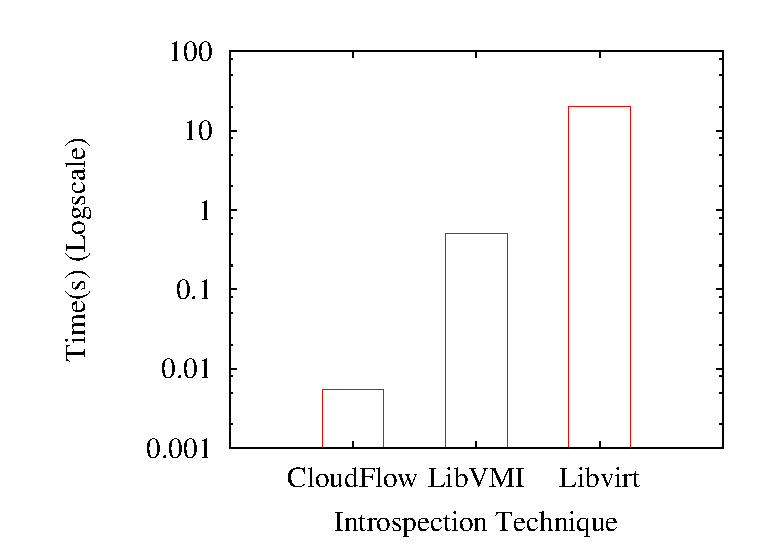
\includegraphics[scale=0.6]{figures/introspectionwindow.eps}
%\vspace{30pt}
\caption{\small 
%
CloudFlow features a low impact introspection design that allows it to
perform significantly faster than existing introspection libraries.  The
shorter the introspection cycle, the smaller the window of vulnerability
during which a VM can be attacked.
% 
\label{cloudflow:figure:introspectionwindow}}
\end{center}
\end{figure}

\begin{figure}[t]
\begin{center}
\includegraphics[scale=0.6]{figures/guestslowdown.eps}
%\vspace{30pt}
\caption{\small 
%
CloudFlow has a minimal overhead, below 2\% slowdown in guest workloads. 
Performance slowdown caused by CloudFlow remains well within the normal
variation shown by typical workloads, represented here by the error bars. 
%
\label{cloudflow:figure:guestslowdown}}
\end{center}
\end{figure}




%Evaluation
\vspace{5pt}

\section{Evaluation}
\label{sec:evaluation}

We now explore two different performance aspects of CloudFlow. 
The first aspect is the ability to minimize the window of time during which
a particular VM remains vulnerable to side channel attacks, after it has
started a security-critical workload.  CloudFlow provides a best-effort
solution and only a small window of vulnerability exists where the victim
can be targeted.  The aim of the experiments is to find out exactly how
small this window is.  The second aspect is the performance slowdown
experienced within the guest due to constant introspection.  Our
introspection technique is polling based and causes a constant but minimal
overhead.  Finally, VMs may undergo dynamic migration for policy conflict
resolution and resultant latency causes the guest to perform
slower.  We minimize the impact of this overhead by scouting out conflict-free migration targets.

\noindent
{\bf Specs.~} 
% 
2.90 GHz Intel i7-3520M nodes with 4GB memory running 64-bit Ubuntu 12.04.1
LTS.  The VMs are running 64-bit Fedora 16 with 2GB of memory. The benchmark
suite of choice was the Phoronix Test Suite \cite{Phoronix}.

\noindent
{\bf Vulnerability Window.~}
%
Since CloudFlow is reactive in nature, a major aim is to minimize the window of
vulnerability during which an attack can be mounted against a target VM. 
The size of this window is precisely the time it takes from the moment a
security critical workload starts to run to the moment an appropriate policy
enforcement is executed.  Whenever a runtime label matches a policy
that needs to be enforced CloudFlow freezes the VM. As CloudFlow performs continuous introspection, the vulnerability window
is exactly the wall-clock time it takes to do a complete introspection cycle over the
required kernel data structures.

In an initial version of CloudFlow we started using libvirt \cite{libvirt} 
and libVMI \cite{libvmi} as the libraries of choice for KVM-QEMU
introspection.  It became quickly apparent that these libraries are not
designed for low-latency response and the combination is unusable for
meaningful real-time introspection. 
%
% The reason for this turned out to be unnecessary socket communication used for
% IPC within the library and long delays caused by the KVM-QEMU messaging
% systems used to communicate with KVM-QEMU.  
%
Instead, we wrote our own custom fast introspection interface for KVM-QEMU
which sheds all unnecessary libvmi/libvirt overheads and runs within
KVM-QEMU as a thread that can use KVM-QEMU internals directly to read guest
memory.  This allowed us to {\em perform orders of magnitude faster that
existing techniques}.  As shown in Figure
\ref{cloudflow:figure:introspectionwindow}, CloudFlow only takes around
4.7ms wall clock time (less than 2\% of which is CPU time) to perform one
complete pass over all the desired kernel structures.  This figure was
achieved for >50 guest processes running -- the behavior does not vary
significantly with increasing number of processes.



\noindent
{\bf Performance.~}
%
CloudFlow is broken down into independently functioning components that
communicate with each other asynchronously.  Out of all the components, the
most computationally intensive module is the introspection module.  The
introspection runs as a thread inside of KVM-QEMU and as a result affects
the runtime performance of the monitored guests.  Figure
\ref{cloudflow:figure:guestslowdown} shows the runtime performance of the
guest operating system with both introspection on and off (lower is better). 

The slowdown caused by CloudFlow introspection is upper bound around 1.7\%
above the baseline performance measured with introspection turned off. 
CloudFlow performs well within the original error bounds of the baseline
performance. All
other components run separately and do not cause any performance impact for
guest workloads.

%Guest performance with introspection on and off (Use Phoronix test suite to do a bunch of tests here. Current ideas: Apache Run, Apache compile, (other computationally intensive tasks). The idea is guest performance should slow down due to constant introspection but we want to show the slowdown is not enormous.

\noindent
{\bf Migration Cost.~}
% 
Finally, the guest VM is also subject to dynamic migration in the case of a
policy conflict.  Whenever this situation arises, the latency of migration
causes a performance hit for the guest.  For our experimental setup, time
taken to do a single migration hovers around the 20 seconds mark -- however
this figure is likely to vary wildly depending on network load, utilized RAM
and volume/disk persistence models (reconnection of volumes to the migrated
VM takes time).  Although frequent migration of VMs impedes user experience, it is important to note that in most
policies, migration likely gets triggered only when a security critical
service launches and the VM relocated is mandated by a policy impacting it. The
non-cloud alternative of having an entire separate machine dedicated to each
individual task is most likely much more expensive.



%Conclusion and Future Work
\section{Conclusion and Future Work}
\label{sec:conclusion}

%\begin{enumerate}
%\item Summarize the problem we solved.
%\item Restate all our contributions that were mentioned in the introduction and say how our results really back up our contributions.
%\item Mention some future directions (that are non-trivial)
%\end{enumerate}

The main contributions of this paper include (i) a new introspection
mechanism for the KVM-QEMU \cite{QEMU} hypervisor that allows for fast
asynchronous virtual machine introspection at the hypervisor level, orders
of magnitude faster than previous approaches, and (ii) a cloud wide
information flow control layer for OpenStack \cite{OpenStack} that leverages
the introspection mechanisms to enforce best effort real-time information
flow control.


% We have restricted our runtime labels to conform to SELinux types and
% focused on the policy enforcement infrastructure rather than developing
% complicated label sets.  One exciting avenue for future work is enhancing
% CloudFlow to handle an arbitrary set of labels inside the guest VM.  The
% introspection module can be augmented with schemes that look at larger parts
% of the guest memory (as opposed to data structures used in this paper) and
% use this data to provide the same information flow control invariants for an
% environment where the guest operating system is potentially untrusted.

Ongoing and future work includes (a) new stronger introspection mechanisms
resilient to malicious guest OSes and (b) CloudFlow extensions that will
allow policies to be written in terms of additional guest state elements,
including I/O state, intra-OS events and IPC. 



\bibliographystyle{plain}
\bibliography{bib/refs}

%\input{appendix.tex}


\end{document}
